\documentclass[11pt,a4paper,titlepage]{report}
\usepackage[utf8]{inputenc}
\usepackage[english]{babel}
\usepackage[margin=1in]{geometry}
\usepackage{amsmath}
\usepackage{amsfonts}
\usepackage{amssymb}
\usepackage{url}

\usepackage{graphicx}
\usepackage[justification=centering]{caption}
\usepackage{qtree}
\usepackage{dirtree}
\usepackage{bytefield}

\linespread{1.24} %riviväli 1.5
%\sloppy % Vähentää tavutuksen tarvetta, "leventämällä" rivin keskellä olevia välilyöntejä.

\renewcommand{\thesection}{\arabic{section}}


\author{Group 8\\Niko Hellgren, 505174}
\title{BGP Simulator Documentation}
\date{Protocol Processing, Spring 2017}

\begin{document}
\maketitle
\tableofcontents
\pagebreak

\section{Project specifics}\label{sec:project}
\begin{figure}
\begin{center}
\begin{tabular}{r l}
\textbf{Time taken} & \textbf{Description}\\
9 h & Implementing the classes for BGP message types \\
2 h & IPv4 packet implementation \\
3 h & Routing table, initial implementation \\
4 h & Router initialization, designing structure \\
4 h & Implementing BGP message handling \\
4 h & Implementing router handshake \\
3 h & Implementing \texttt{UPDATE} message handling \\
6 h & Routing table, complete rewrite \\
2 h & Notification message generation and exception throwing \\
5 h & Trust system, cryptographically protected voting \\
2 h & Client implementation and behaviour \\
10 h & Fixing issues
\vspace{3mm} \\
15 h & Writing the report \\
3 h & Doing the presentation \\
\hline
\textbf{75 h} & \textbf{Total time (approx.)}
\end{tabular}
\end{center}
\caption{Approximate list of time taken by various parts\\of the project, semi-chronological ordering.}
\label{fig:timetaken}
\end{figure}

This document and the corresponding source code are done as a course project for course Protocol Processing, held in University of Turku in spring of 2017. I did the project by myself (and therefore there is no attached work distribution table), an approximate time-distribution of the various tasks is presented in Figure \ref{fig:timetaken}. I started as a part of another group, but the large size on the group and my will to gain knowledge and experience on all parts of the implementation caused me to extract myself from the previous group. As an afterthought, that was a really good idea, and gave me an excellent possibility to both learn specifics on network routing and do a semi-large ($\sim 5000$ LoC) programming project by myself. Initially being a member of a group delayed starting the project by about two weeks. Since there was no need to communicate the specifics of the implementation to other people during implementation, the planning went on mostly as a thought process, and the first implementation of most classes was on source code.

The initial plan was to implement each router and its contained functionalities (routing table, connections, trust) as separate objects running their own threads, and implement the physical and data link layers of the connections between routers using some of Java's built-in stream classes, due to their good support for multi-thread implementations. The first idea of the routing table was using two tree structures: one for known subnets (presented in \ref{sec:routing}) and one for connections between routers in the network. This dual model worked rather well, until I realized there was no way to know when a link between two routers is broken, the \texttt{UPDATE} message only tells what subnets are no longer reachable. This required a complete rewrite of the routing engine. Outside the problem with the routing table implementation, the whole process was rather straightforward, and no major issues were encountered.

The largest issues during the project stemmed from the definition of BGP \cite{RFC4271} focusing only on the limitations and requirements of the protocol, not so much on the implementation. Most attempts at finding information on the implementation yielded only information on how to do a specific action on a Cisco router. Apparently, implementing a BGP router is not a very common task, and the best practices of the field are hard to come by.

From design point-of-view, the visualization of the network and the simulation was the hardest part. Implementing a functioning GUI would be the best solution, but that would, naturally, take a long time. For the final implementation, I settled for a text-based configuration with a graphical representation of the network.

\section{Introduction}\label{sec:intro}
The simulator software is implemented in Java programming language using just the base libraries. For visualization purposes, a graph plotting library, GraphStream \cite{graphstreamteam2017}, was attached. A high-level overview of the program structure is presented in Section\ref{sec:hlo}. The code is available in \url{https://github.com/nipehe/BGP-simulator} for the time being.

The simulation has the following basic technical features and limitations:
\begin{itemize}
\item The simulation is strongly threaded, with each router and client working as its own thread and \texttt{Timer} threads utilized in testing and \texttt{KEEPALIVE} messages.
\item Layer 1 and Layer 2 functionalities are simulated by Java's \texttt{PipedInputStream} and \texttt{PipedOutputStream} that are made to transit \texttt{byte[]} arrays between threads. The output streams are \texttt{synchronized} to make sure the sent packets do not mix up.
\item Layer 3 functionality is implemented according to the IPv4 protocol. Although the constructed packets contain and transmit all the fields defined in \cite{RFC0791}, fields \emph{Type of Service}, \emph{Identification}, \emph{Flags}, \emph{Fragment Offset}, and \emph{Protocol} are filled with default values in all cases, and they are not used for anything. This is partly enabled by the simulation not supporting packet fragmentation.
\item A globally available static class provides the simulated routers and clients with DNS-like functionality, since implementing an actual DNS functionality is not essential in this simulation.
\item To provide packets for the simulation, clients are attached to the router objects and they have functionality to send data to each other over the network.
\item The simulated network uses BGP-4 messages to transmit information between routers.
\item Since the simulation is focused on BGP, the idea of Autonomous Systems (AS) is abstracted into each AS being represented by one router, and the clients attached to this AS being connected straight to the router. This removes some features concerning, for example, the \texttt{NEXT\_HOP} attribute, since the hops done are always to another AS/router.
\item TCP functionality is not implemented, and BGP packets are transmitted as ordinary IP packet payloads. This removes the possibility to test or simulate security and stability issues caused by TCP, and simplifies the connection process, but streamlines the implementation due to the complicated specification and functionality of TCP \cite{RFC0793}.
\item Routing information is transmitted using \texttt{UPDATE} messages after connection initialization and all routing table changes.
\item Additional BGP message type, \texttt{TRUST} has been added for trust voting between routers. To avoid Man-in-the-Middle attacks (usually the router being voted on is on the transmission path of the vote), the trust votes are encrypted using 1024-bit RSA and signed using RSA with SHA-1. To avoid making key transmission overly complicated, a PKI-like functionality was made available as a globally available class, providing routers with other routers public keys. The trust implementation is discussed in more detail in Section \ref{sec:trust}.
\item Behaviour in error situations has been implemented comprehensively, and both L1/L2 breakage, missing \texttt{KEEPALIVE} messages, and erroneous BGP messages cause the routers to drop the link and inform their neighbourhood of this. Possible issues effect the trust rate of the misbehaving router.
\item Since the simulation is targeted at demonstrating the behaviour of BGP, logging has not been implemented.
\end{itemize}

\section{Code overview}\label{sec:hlo}

\begin{figure}
\dirtree{%
.1 bgp.
.2 client\DTcomment{Clients of simulator's routers}.
.3 messages\DTcomment{Messages transmitted between clients}.
.2 core\DTcomment{Router implementation}.
.3 messages\DTcomment{BGP message implementations}.
.4 notificationexceptions\DTcomment{Exception classes used to notify about situations that should raise a \texttt{NOTIFICATION}}.
.4 pathattributes\DTcomment{Path attributes used in \texttt{UPDATE} messages}.
.3 network\DTcomment{Network adapter simulation, L1/L2 functionality}.
.4 fsm\DTcomment{Finite state machine used by the inter-router connections}.
.4 packet\DTcomment{Interfaces defining behaviour for actors handling packets}.
.3 routing\DTcomment{Routing table engine}.
.3 trust\DTcomment{Inter-router trust table}.
.2 tests\DTcomment{JUnit tests to ensure correct working of the program}.
.2 ui\DTcomment{User interface components}.
.2 utils\DTcomment{Functionalities needed by various classes (e.g. IP addresses)}.
}
\caption{Package structure of the code}
\label{fig:packagestructure}
\end{figure}

\begin{figure}
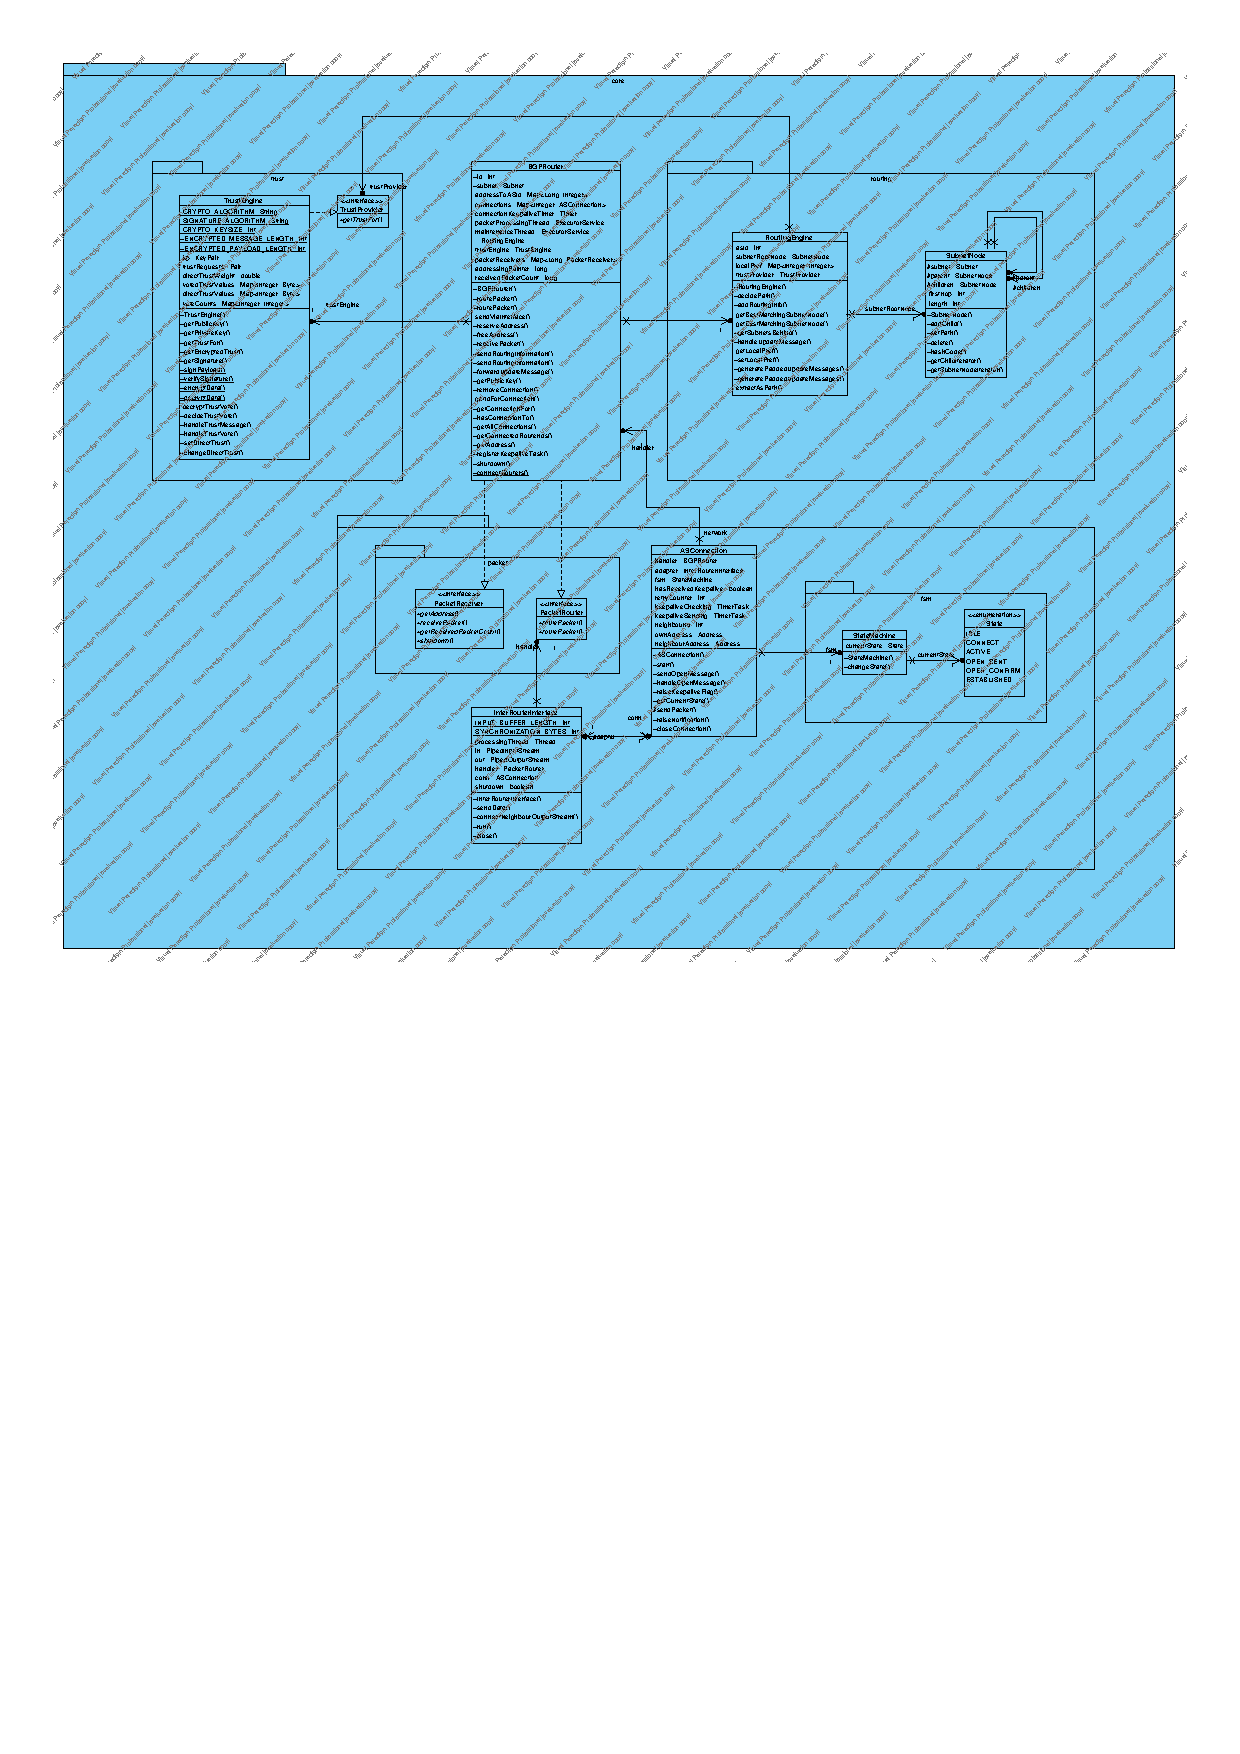
\includegraphics[width=\textwidth]{uml_1}
\caption{UML diagram of the router's main classes}
\label{fig:uml}
\end{figure}

This section discusses the code-level decisions and structure in the project. Smaller details are overlooked, and the focus is on main functional parts of the program. A package-level visualization of the project can be found in Figure \ref{fig:packagestructure}.

\paragraph{\texttt{bgp.core.SimulatorState}}
Global state to transmit information between parts of the simulation that is either not possible or relevant to transmit via the network. This contains registry of the routers and clients (with checks for duplicate ID's), DNS-like functionality that provides information about client's addresses for data transmission purposes, and PKI-like functionality that provides routers' public keys used in trust voting.

\paragraph{\texttt{bgp.core.BGPRouter}}
Objects from this class represent the routers that make up the network. Each router is given an ID (AS ID) and a specified subnet. Routers have a list of \texttt{ASConnection}s that represent the connections to the router's neighbours. Each router also has their own \texttt{RoutingEngine} and \texttt{TrustEngine}, responsible for routing table upkeep and neighbour trust calculations, respectively. The routers implement a DHCP-like behaviour, where they provide clients with IP addresses. To avoid maintenance packets blocking the routing, there are two threads in each router: one for making packet routing decisions and one for processing BGP packets designated to current router. Despite this separation, BGP messages are transmitted via the same media as ordinary routed packets. \texttt{BGPRouter} also has functionalities that bind the features of routing and trust engine and various \texttt{ASConnection}s together.

\paragraph{\texttt{bgp.core.ASConnection}}
Class responsible for storing information concerning the state of a connection from one router to another. Contains the BGP finite state machine, information about this connection's IP address, and a reference to its \texttt{InterRouterInterface}. Is responsible for sending \texttt{OPEN} and \texttt{KEEPALIVE} messages and handling events that require sending a \texttt{NOTIFICATION}.

\paragraph{\texttt{bgp.core.network.InterRouterInterface}}
Represents the L1/L2 functionalities responsible for transferring data between routers. Contains a \texttt{PipedInputStream} and \texttt{PipedOutputStream} for transferring \texttt{byte[]} arrays with the connected neighbour, and a thread responsible for listening the input stream. Sending a packet consists of sending 10 bytes (0x00, 0x00, ..., 0x00, 0xFF) for synchronization and marking the beginning of transmission (not necessary in simulation environment), 2 bytes representing the length of the upcoming packet (MTU is therefore 64 kilobytes), and finally the IP packet as bytes.

\paragraph{\texttt{bgp.core.routing.RoutingEngine}}
Handles \texttt{UPDATE} messages, decides the routing paths and keeps up the routing table. The routing engine behaviour is discussed in more detail in Section \ref{sec:routing}.

\paragraph{\texttt{bgp.core.trust.TrustEngine}}
Calculates trust values for neighbouring nodes based on received \texttt{TRUST} messages and user-defined direct trust, creates \texttt{TRUST} requests and votes with cryptographic protections in place. Trust functionality is presented in Section \ref{sec:trust}.

\paragraph{\texttt{bgp.core.messages.BGPMessage}}
This class, together with its subclasses \texttt{OpenMessage}, \texttt{KeepaliveMessage}, etc., is used to construct BGP messages and serialize them to bit-level representation, and de-serialize them to be used by the receiving end. De-serialization phase is also responsible for message validation.

\paragraph{\texttt{bgp.client.BGPClient}}
Class representing a client of the network, connected through one of the routers. Clients have their own IP addresses and are capable of receiving IP packets. To test network functionality, a ping request and response have been implemented.

\paragraph{\texttt{bgp.utils.Address}}
\texttt{Address}, together with its subclass, \texttt{Subnet}, represent IP addresses and and subnets, respectively, and can be converted into both 4-\texttt{byte} array representation and a 64-bit \texttt{long} representation (\texttt{long} was used instead of 32-bit \texttt{int} to avoid the 1st bit, sign, affecting possible comparisons of addresses). Subnets also store the length of the prefix in question as a bitmask.

\paragraph{\texttt{bgp.utils.PacketEngine}}
Functionalities regarding the construction, validation and modification of IP packets. Packet constructions and verifications, checksum calculations, TTL modifications and field extractions are done here. As mentioned in Section \ref{sec:intro}, Version, IHL, DSCP, ECN, protocol and fragmentation fields are used, but filled with default values.


\section{Connection initialization process}\label{sec:init}
The connection process of two routers is started with a static method, \texttt{BGPRouter.connectRouters}, that connects the \texttt{InterRouterInterface} adapters of the two routers (analogous to connecting the routers via a cable) and starts the process on both ends. After this, the two routers continue the process independently. On both ends, the process goes as follows:
\begin{enumerate}
\item Change the finite state machine in the \texttt{ASConnection} to state \texttt{CONNECT}, reset the retry counter.
\item Send an \texttt{OPEN} message, retry if necessary. Change the FSM state to \texttt{OPEN\_SENT} or raise a notification if unable to send the message.
\item Wait for an \texttt{OPEN} message from the other router. This process is independent of the earlier steps, so an \texttt{OPEN} message can be received before one has been sent. If current state is \texttt{CONNECT} or \texttt{OPEN\_SENT} when the \texttt{OPEN} message is received, start sending and checking for \texttt{KEEPALIVE} messages, and change the FSM state to \texttt{OPEN\_CONFIRM}.
\item The scheduled \texttt{KEEPALIVE} checking task checks whether current state is \texttt{OPEN\_CONFIRM}, so once it has received the first \texttt{KEEPALIVE} message, it can change the current state to \texttt{ESTABLISHED} and send initial routing information to the other end. Until the state has been changed to \texttt{ESTABLISHED}, the connection can not be used to transmit ordinary IP packets.
\item Build initial \texttt{UPDATE} messages that send the whole local routing table to the other end. To ensure correct route lengths, the \texttt{AS\_PATH} field is padded with own ID, and a different \texttt{UPDATE} message is constructed for each differing path length.
\end{enumerate}

\section{Routing engine}\label{sec:routing}
This section presents the routing engine used to make routing decisions and handle \texttt{UPDATE} messages. The decision process on receiving an \texttt{UPDATE} message is discussed first, with behaviour on link breakage and route selection presented after that.

\subsection{Decision process}\label{ssec:decision}
Upon receiving a new \texttt{UPDATE} message, the routing engine validates it and then follows the following algorithm:
\begin{enumerate}
\item Iterate over the withdrawn routes (if present):
	\begin{itemize}
	\item If exactly matching routing information is not found, do nothing.
	\item Else, if the first hop on the \texttt{UPDATE} message matches the current best path for the subnet, remove the routing information for the subnet and store the subnet to be sent to other neighbours (if currently revoking neighbour was not on the best path, it is not necessary to inform neighbours of this, since it is not on the best path from this router).
	\item Else store the information about the subnet and selected best path to it. This collection of non-removed subnets will be replied to the revoking peer to inform it of a possible alternative route through this router.
	\end{itemize}

\item Iterate over the Network-layer reachability information (if present):
	\begin{itemize}
	\item If no exact match to the subnet in question is found from the current routing table, create a new node and insert it into the correct location on the subnet tree, with first hop, path length and local preference information based on the path attributes.
	\item Else if the local preference values of the current and possible new path differ; store/keep the better selection in the tree.
	\item Else, store the shorter path scaled with trust values of the neighbours (presented in detail in Subsection \ref{ssec:trustcalc}).
	\item If the selected path was changed, store it for sending to other neighbours.
	\end{itemize}
	
\item Modify the received \texttt{UPDATE} message\footnote{\texttt{NEXT\_HOP} value is changed before serializing the message for each neighbour.}:
	\begin{itemize}
	\item Add own ID to the beginning of \texttt{AS\_PATH}.
	\item Remove routes that were not used from Withdrawn routes list.
	\item Remove NLRI entries that were not utilized by this router.
	\end{itemize}

\item Send the modified message to each neighbour not in the \texttt{AS\_PATH}.\footnote{Since changes not affecting routing decisions are not propagated, the original \texttt{UPDATE} message content diminishes as the information travels further in the network.}
\item Send information about revoked subnets reachable via this router to the revoking neighbour.
\end{enumerate}

\subsection{Route withdrawals}
If a connection to a neighbour is broken, an \texttt{UPDATE} message with all subnets that were originally reached via that neighbour attached to the Withdrawn routes list. This message is then handled according to the algorithm defined in \ref{ssec:decision}, thus removing the routing information and sending the information to all neighbours. Due to the reply feature defined in the decision process algorithm, if an alternative route exists, information about that should reach the router originally revoking connections, after the information has reached a router that has a differing best path.

\subsection{Subnet tree}
\begin{figure}
\Tree [.0.0.0.0/0 [.0.0.0.0/1 [.$\vdots$ [.10.0.0.0/8 $\vdots$ $\vdots$ ] [.11.0.0.0/8 $\vdots$ $\vdots$ ] ] $\vdots$ ] [.128.0.0.0/1 $\vdots$ [.$\vdots$ [.192.168.100.0/24 $\vdots$ $\vdots$ ] [.192.168.101.0/24 $\vdots$ $\vdots$ ] ] ] ]
\caption{Tree structure used to categorize the subnets}
\label{fig:subnettree}
\end{figure}

Subnets in the 32-bit IPv4 address space can be categorized into a binary tree, with each level having prefix length one longer than the previous one (see Figure \ref{fig:subnettree}). For the purposes of the routing engine, the binary tree was not complete, but was instead populated with all the prefixes received as Network-layer reachability information (NLRI), placing each new node in the graph as a child of the longest prefix containing the new subnet. Each node contains information about the first hop to be taken to get on the currently selected path to the target subnet, local preference of the currently selected first hop and the length of the path to the goal node. The graph is started with a single node with the prefix 0.0.0.0/0, with first hop set to be the default route, if specified\footnote{Not specifying a default route causes the packets that are not designated to any known subnet with a prefix longer than 0 to be dropped.}.

\subsection{Route selection}
Route selection is achieved by first finding the longest matching subnet by recursively looking through the subnet tree, continuing deeper into the tree as long as a child subnet node that contains the address being looked for is found, and then extracting the first hop ID from the node representing the longest matching prefix. \texttt{BGPRouter} has a map from neighbour's ID to the corresponding \texttt{ASConnection}, which can then be used to transmit the packet. If the longest matching prefix is the current router's subnet, local routing is done to either one of the clients or the router itself.

\section{Trust implementation}\label{sec:trust}
The mechanism responsible for deriving the amount of trust placed upon a neighbour could be considered to be a simplified version of the solution by Rantala et al. \cite{DBLP:journals/corr/abs-1105-5518}. Each router defines an overall trust rate to each of its neighbours based on direct trust, consisting of inherent trust (specified by the operator) and observed trust (specified by neighbour's behaviour), and voted trust, with specifiable emphasis on either part.

\subsection{Calculating trust}\label{ssec:trustcalc}
Each router holds two trust values for each neighbour: inherent trust and voted trust, with voted trust initially at 0 (range $-128..127$ for easier transmission) and inherent trust at value specified by the operator. The total trust value is derived from these values as a weighted sum. For path selection purposes, this value is scaled to range $0..1$, and used to derive a \emph{normalized routing criterion with trust rate}, as originally presented by He \cite{1690485}:
\[
C_T=\frac{C}{T} \text{, where } C=\text{initial cost (in this case, path length), } T=\text{trust rate}
\]

\subsection{Modifying trust}\label{ssec:trustmod}

Modifying the inherent trust can either be done by the operator or automated observations of the neighbours behaviour. In the current implementation, negative behaviour (dropping connection, sending invalid BGP messages) lowers the observed trust rating, while continuous normal behaviour raises it.

Voted trust is changed by second-order neighbours' votes, and is defined as the average of received votes. For a more robust solution, second-order neighbours' trust values could also be defined, using them as weights for average calculation.

\subsection{Voting on trust}\label{ssec:trustvote}

\begin{figure}
\begin{center}
\begin{bytefield}[bitwidth=1.1em]{32}
\bitheader{0-31}\\
\bitbox{1}{T} \bitbox{7}{}
\bitbox{16}{Reviewer AS ID}
\bitbox{8}{Target AS ID (1/2)}\\
\bitbox{8}{Target AS ID (2/2)} \bitbox[lrt]{24}{}\\
\wordbox[lr]{2}{Encrypted vote (128 bytes, only if T=1)}\\
\skippedwords\\
\bitbox[lrb]{8}{} \bitbox[lrt]{24}{}\\
\wordbox[lr]{2}{Vote signature (128 bytes, only if T=1)}\\
\skippedwords\\
\bitbox[lrb]{8}{} \bitbox[lt]{24}{}
\end{bytefield}
\end{center}
\caption{\texttt{TRUST} message structure}
\label{fig:trust}
\end{figure}

Current implementation asks for trust votes from second order neighbours every time an \texttt{UPDATE} message with more than one router in the \texttt{AS\_PATH} is received. This is done by sending a \texttt{TRUST} request BGP message (presented in Figure \ref{fig:trust}). The first bit, type, specifies whether the message is a vote request (T=0) or vote response (T=1). The rest of the bits in the first octets are empty, and usable in future extensions. Following four octets specify the reviewing router ID (2 octets) and the ID of the router being voted on (2 octets).

After the initial fields comes the payload of the message. If the message is a vote request, the payload field is empty, and otherwise it consists of the (encrypted) vote value and a signature for verification purposes. The vote value is 128-bytes long, and it is derived by encrypting the inherent trust value and 116 random bytes (the random values are appended to increase the message length, and therefore limiting brute-force attacks against the encryption) using 1024-bit RSA encryption. The signature is generated from the encrypted vote payload using RSA with SHA-1. The same key pairs are used for both encryption and signing purposes, and the public keys are distributed by \texttt{SimulatorState}.

Upon receiving a \texttt{TRUST} message, the router checks the type, and depending on it either constructs a response or modifies the voted trust based on the received vote. If the type of the received message was 0, the response is constructed by setting the type bit to 1, adding own ID and target ID as the next four octets, generating a 117-byte message with 1st byte representing the \emph{inherent} trust towards the target router, encrypting the message, creating a signature of the encrypted payload and appending both of these to the message. If the type is 1, the router first checks that a trust vote request was actually sent by removing a corresponding token from the list of requests, if present. Then, the correspondence of the signature and the payload is checked using the public key of the voting party (received from the \texttt{SimulatorState}) and, if the signature matched, the encrypted vote is decrypted and the value of the first payload octet is used to modify the voted trust.

\section{Topics for future development}\label{sec:future}
The limited time (10 weeks) and group size (1 person) affected the possibilities of the implementation somewhat. This section considers features and extensions the simulation could benefit from but what could not be implemented this time.

From information security perspective, implementing the TCP layer functionality would increase the possible attack surface and make the simulation more realistic. Another interesting feature, that would also defer the vulnerabilities of aforementioned TCP, would be a separate control layer to transfer BGP messages. Without the need for extensive cabling or other transmission media, this would be really viable in a simulation environment.

Adding a random possibility of error to the data transmission (dropping bytes, switching bits) would strain error-correction features, but since none are implemented (IP headers are validated, payload is not), this would cause unfixable erroneous behaviour in the simulation. Since the L1 transmission is done over Java's \texttt{PipedInputStream}s and \texttt{PipedOutputStream}s in the same process, the current chance of error due to erroneous transmission is close to non-existent.

Current implementation of the decision process only stores the currently selected path for each subnet. Holding multiple possible routes and balancing the load on them would lessen the workload of routers along the best path to a specified router. As a side-effect, current implementation does keep the packets in the right order, since there is only one thread routing packets in each router, and all packets going between the same two routers use the same route. In case of a link going down, a router also needs to wait for alternative route information from other routers in the network, before being able to route packets to the wanted network again.

\section{Miscellaneous technical notes from the project}\label{sec:notes}
\begin{itemize}
\item When Java interprets bytes as numbers, they are shifted to range -128..127, using the first bit as a sign bit. Doing bitwise shifts also easily converts the values to a larger data size (e.g. 32-bit integers) instead of dropping the overflowing bits. This caused multiple errors in initial implementations of the bit-level manipulations, and adding bitmasking (e.g. \texttt{<value>\&0xFF} to force a value to 8 bits) was necessary in most of the places to avoid issues caused by this. Lack of unsigned numbers also made value comparisons difficult at some points, since the interpretations of bytes easily flowed over to the negative numbers.
\item Great built-in support for threads, timers and task executors in Java 8 made some otherwise difficult tasks (e.g. \texttt{KEEPALIVE} message sending and checking) really easy.
\item Following object-oriented paradigm in development was both intuitive and helpful, mostly due to the software being a simulator.
\end{itemize}

\bibliography{documentation}
\bibliographystyle{ieeetr}

\end{document}